\subsubsection{Интерполяция на четырехугольном КЭ}
\paragraph{Билинейная интерполяция}
Пусть в четырёх узлах КЭ (обозначены красным) $Q_{11}, Q_{12}, Q_{21}, Q_{22}$ с координатами $x_1, y_1; x_2, y_2; x_3, y_3; x_4, y_4;$ значения исходной функции известны. Требуется получить приближённое (интерполированное) значение исходной функции в точке $P$ (обозначена зеленым) с координатами $x, y$ (см. Рисунок \ref{Bilinear_interpolation}).
\begin{figure}[H]
	\centering
	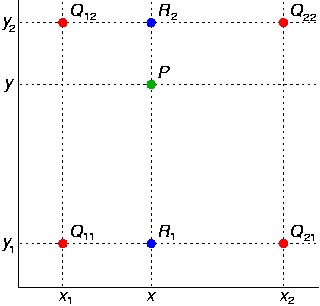
\includegraphics[width=0.4\linewidth]{img/Bilinear_interpolation}
	\caption{Постановка задачи билинейной интерполяции}
	\label{Bilinear_interpolation}
\end{figure}
Первым шагом линейно интерполируется значение вспомогательных синих точек $R_1, R_2$ (обозначены синим) вдоль оси абсцисс, где
\begin{equation*}
	R_1 = (x,y_1),\quad R_2 = (x,y_2),
\end{equation*}
тогда
\begin{equation*}
	\begin{array}{cc}
		f(R_1)\approx \tau f(Q_{11}) + (1-\tau)f(Q_{21})\\
		f(R_2)\approx \tau f(Q_{112}) + (1-\tau)f(Q_{22})
	\end{array}\quad
	\tau = \frac{x_2-x}{x_2-x_1}
\end{equation*}

При вычислении $\tau$ по данной формуле в четырехугольном КЭ отличном от прямоугольника, может получиться $\tau>1$. Чтобы учесть этот случай, будем ограничивать $\tau$ следующим образом
\begin{equation*}
	\tau = \min\left\{1,\, \frac{x_2-x}{x_2-x_1}\right\}.
\end{equation*}

Теперь проводится линейная интерполяция между вспомогательными точками $R_1, R_2$. В результате получаем:
\begin{equation*}
	f(P)\approx pf(R_1) + (1-p)f(R_2)\quad p=\frac{y_2-y}{y_2-y_1}
\end{equation*}
Это и есть интерполируемое значение функции $f(x,y)$, причём значения интерполирующей функции $F(x,y)$ равны значениям интерполируемой функции в исходных точках $Q_{11}, Q_{12}, Q_{21}, Q_{22}$.
\begin{align*}
	f(x,y) \approx F(x, y) = & \frac{f(Q_{11})}{(x_2-x_1)(y_2-y_1)} (x_2-x)(y_2-y)\ + \\
	+                        & \frac{f(Q_{21})}{(x_2-x_1)(y_2-y_1)} (x-x_1)(y_2-y)\ + \\
	+                        & \frac{f(Q_{12})}{(x_2-x_1)(y_2-y_1)} (x_2-x)(y-y_1)\ + \\
	+                        & \frac{f(Q_{22})}{(x_2-x_1)(y_2-y_1)} (x-x_1)(y-y_1).
\end{align*}
Код программы для метода билинейной интерполяции:
\lstinputlisting[language=C++, firstline=7, lastline=36]{current-lines/src/Element/QuadrangleElement.cpp}